\documentclass[crop,tikz]{standalone}

\usepackage[utf8]{inputenc}

\usetikzlibrary{decorations.markings}

%\pic[opts] at (x,y) {torus={R}{r}{alpha} node[opts] <args>;
%pic[opts] can be fill, for example, or rotate. R = outer radius, r = inner radius (R>r), alpha = inclination. node[opts] <args> are standard node commands.
\tikzset{
  pics/torus/.style n args={3}{
    code = {
      \providecolor{pgffillcolor}{rgb}{1,1,1}
      \begin{scope}[
          yscale=cos(#3),
          outer torus/.style = {draw,line width/.expanded={\the\dimexpr2\pgflinewidth+#2*2},line join=round},
          inner torus/.style = {draw=pgffillcolor,line width={#2*2}}
        ]
        \draw[outer torus] circle(#1);\draw[inner torus] circle(#1);
        \draw[outer torus] (180:#1) arc (180:360:#1);\draw[inner torus,line cap=round] (180:#1) arc (180:360:#1);
      \end{scope}
    }
  }
}

\begin{document}

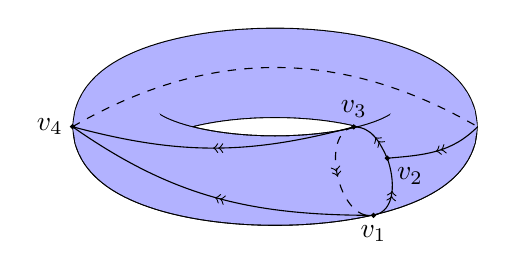
\begin{tikzpicture}

	\pic[fill=white!70!blue] at (0,0) {torus={2cm}{0.56cm}{70}};
	
	\filldraw (1.25,-1.125) circle (.025) node[anchor=north] {$v_1$}; %botton of outer ring
	\filldraw (1.425,-0.4) circle (.025) node[anchor=north west] {$v_2$}; %between v_1 and v_3
	\filldraw (1,-0.00175) circle (.025) node[anchor=south] {$v_3$}; %top of inner ring
	\filldraw (-2.5725,0) circle (.025) node[anchor=east] {$v_4$}; %left side of torus
	
	\begin{scope}[decoration={markings, mark=at position 0.5 with {\arrow{>>}}}]
		%edge on front side of torus linking 2-->3
		\draw[postaction={decorate}] (1.425,-0.4) to[in=0, out=115] (1,-0.00175);
		%edge on front side of torus linking 1-->2
		\draw[postaction={decorate}] (1.25,-1.125) to[in=290, out=10] (1.425,-0.4);
		%edge on reverse side of torus linking 3->1
		\draw[dashed, postaction={decorate}] (1,-0.00175) to[in=190, out=190] (1.25,-1.125); 
		%edge on front side of torus linking 3-->4
		\draw[postaction={decorate}] (1,-0.00175) to[in=345, out=195] (-2.5725,0);
		%edge on front side of torus linking 1-->4
		\draw[postaction={decorate}] (1.25,-1.125) to[in=325, out=180] (-2.5725,0);
		%edge on front side of torus linking RHS to 2
		\draw[postaction={decorate}] (2.5725,0) to[in=5, out=225] (1.425,-0.4);
	\end{scope}
	%edge on reverse side of torus linking 4-->RHS
	\draw[dashed] (-2.5725,0) to[in=180-30, out=30] (2.5725,0);

	
\end{tikzpicture}

\end{document}